\subsection{Sensorbaustein}\label{subsec: Sensorbaustein}
\label{sec: Sensorbaustein}
In diesem Unterkapitel werden die Anforderungen und die Hardware des Sensorbausteins behandelt.
Vom Auftraggeber ist ein Sensorbaustein mit 4-Tasten-Feld und Temperaturfühler gefordert. Der Sensorbaustein wird dabei ähnlich einer Unterputzsteckdose montiert und hat eine WLAN-Schnittelle um die Sensordaten auszulesen. In der Abbildung \ref{pic: Uebersicht_Sensorbaustein} ist die Übersicht des Sensorbausteins dargestellt. Der Baustein wird über ein 5V-Netzteil mit Spannung versorgt, da der Mikrocontroller auf 3.3V läuft, wird mithilfe eines Spannungswandlers die 5 V zu 3.3 V gewandelt. Um den Mikrocontroller zu programmieren steht eine USB zu UART Verbindung, Taster zum Debbuggen, Reseten oder Programmieren und eine Zustands-LED zur Verfügung. Um die Temperatur zu erfassen wird ein NTC verwendet. Da die mitgelieferte Meander-Antenne des ESP32 nur eine kleine Abstrahlleistung hat, kann optional noch eine grössere Antenne, wie z.B. eine zertifizierte grössere Patch-Antenne über RP-SMA angeschlossen werden, falls der ESP32S ausgewählt wird. Der Anwender wird ein Touch-Tastenfeld, sowie dazugehörige LEDs, für die Interaktion mit dem Baustein zur Verfügung haben.  

\begin{figure}[H]
	\centering
	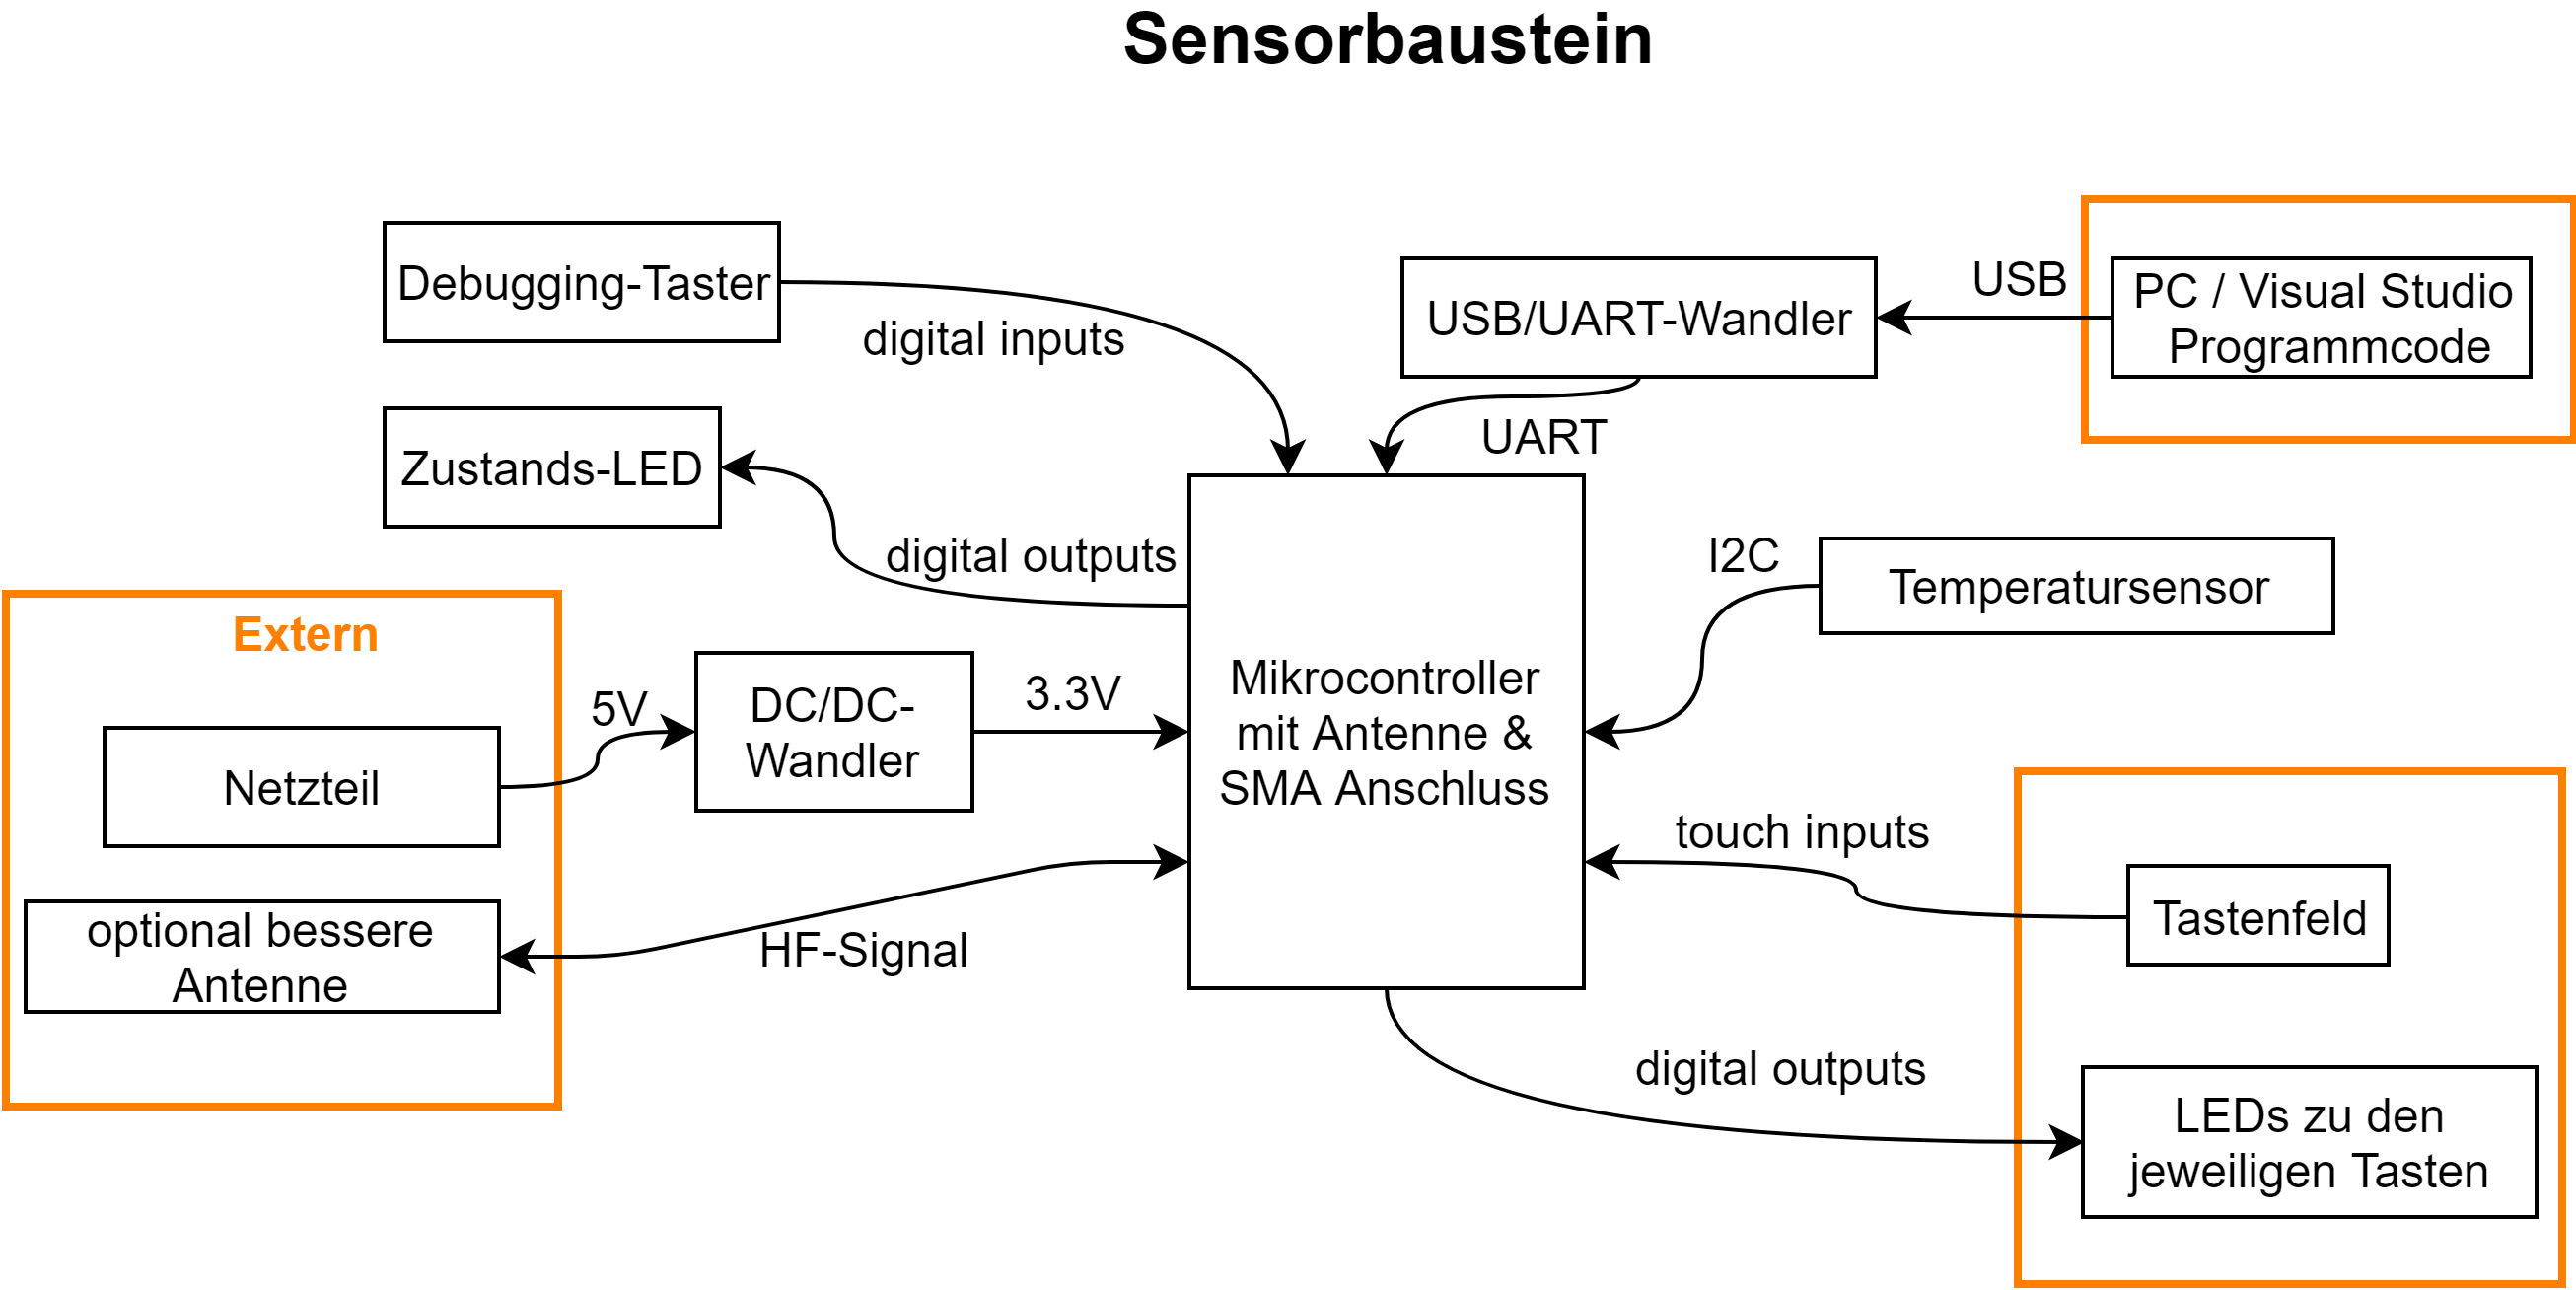
\includegraphics[width=\textwidth]{graphics/Sensorbaustein.png}
	\caption{Übersicht Sensorbaustein}
	\label{pic: Uebersicht_Sensorbaustein}
\end{figure} 

\subsubsection{Mikrocontroller}
\label{Hardware Mikrocontroller_Sensor}
Um die Datenkommunikation über WLAN bereitzustellen wird entweder ein ESP32-WROOM oder der ESP32S, welcher im gleichen Formfaktor zur integrierten Antenne auch einen SMA Anschluss bietet, verwendet. Der ESP32 unterstützt Wi-Fi im Bereich von 2.4 GHz bis ca. 2.5 GHz \cite{espressif_esp32-wroom-32_datasheet_en_2019}. Aus folgender Übersicht sind die zur Verfügung gestellten Ein-/Ausgänge des ESP32 zu entnehmen:
% Please add the following required packages to your document preamble:
% \usepackage{graphicx}
% Please add the following required packages to your document preamble:
% \usepackage{graphicx}
\begin{table}[h!]
	\centering
	\begin{tabular}{|c|c|}
		\hline
		\textbf{Name}                                                                          & \textbf{Anzahl} \\ \hline
		\begin{tabular}[c]{@{}c@{}}Analog-to-Digital Converter (ADC)\\   channels\end{tabular} & 18              \\ \hline
		SPI interfaces                                                                         & 3               \\ \hline
		UART interfaces                                                                        & 3               \\ \hline
		I2C interfaces                                                                         & 2               \\ \hline
		PWM output channels                                                                    & 16              \\ \hline
		Digital-to-Analog Converters (DAC)                                                     & 2               \\ \hline
		I2S interfaces                                                                         & 2               \\ \hline
		Capacitive sensing GPIOs                                                               & 10              \\ \hline
	\end{tabular}
	\caption{I/O Uebersicht}
	\label{tab: IO Uebersicht}
\end{table}
\\
Der ESP32 verfügt über alle benötigten Schnittstellen, die für den Sensorbaustein relevant sind. Im folgenden (Tabelle \ref{tab: IO Sensorbaustein}) sind die Inputs/Outputs des Mikrocontrollers (folglich Abb. \ref{pic: ESP32_sensor}), welcher im Sensorbausteins verwendet wird, aufgeführt:
\begin{table}[h!]
	\centering
	\begin{tabular}{|c|c|}
		\hline
		\textbf{Name}                                                                          & \textbf{Anzahl} \\ \hline
		digital outputs für LEDs                                                               & 5               \\ \hline
		digital inputs für Buttons                                                             & 3               \\ \hline
		\begin{tabular}[c]{@{}c@{}}Capacitive sensing GPIOs für Touch\\   Buttons\end{tabular} & 4               \\ \hline
		UART interface für Programmierung                                                      & 3               \\ \hline
		I2C interfaces für Temperatursensor                                                    & 3               \\ \hline
	\end{tabular}
	\caption{I/O Sensorbaustein}
	\label{tab: IO Sensorbaustein}
\end{table}
\\
\begin{figure}[h!]
	\centering
	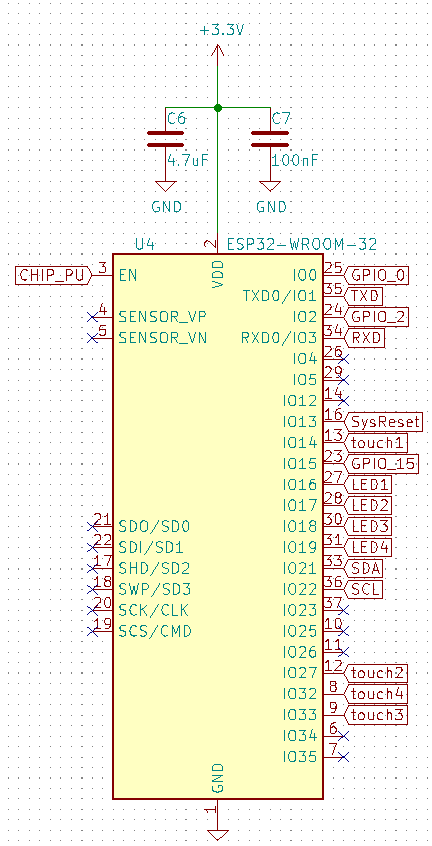
\includegraphics[width=0.5\textwidth]{graphics/shematics_sensor_ESP32.png}
	\caption{Mikrocontroller ESP32 im Sensorbaustein}
	\label{pic: ESP32_sensor}
\end{figure}
\subsubsection{Temperatursensor}
Es wird der TMP1075 verwendet, welcher ein I2C Temperatursensor ist. Dieser hat den Vorteil gegenüber einen rein analogen PTC oder ähnliches, dass er die Temperatur selbständig ermittelt und der Mikrocontroller diese Temperatur nur noch abfragen muss. Preislich sind beide Arten von Sensoren günstig, wobei der TMP1075 0.97 Fr. und im Vergleich der herkömmliche  PTC TMP63GT9Z 1.37 Fr. bei Mouser kostet. Im Bild \ref{pic: Temperatursensor} ist die verwendete Temperatuschaltung abgebildet. Die I2C Adresse des Temperatursensors wird mithilfe von A0, A1 und A3 eingestellt, wobei die eingestellte Adresse in Bild \ref{pic: Temperatursensor} "1001000" lautet.  
\begin{figure}[h!]
	\centering
	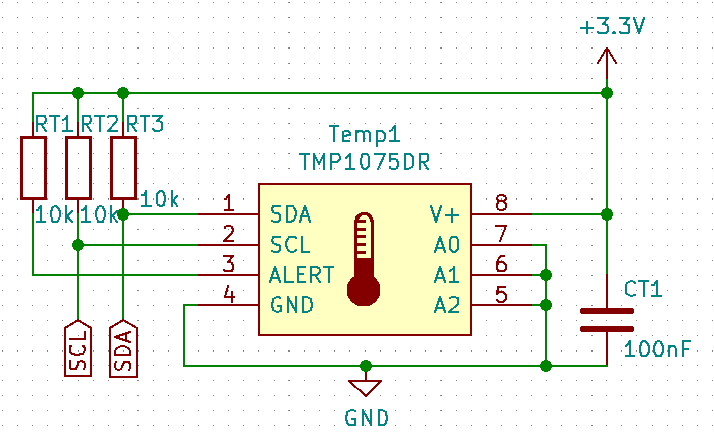
\includegraphics[width=0.5\textwidth]{graphics/shematics_sensor_Temp.png}
	\caption{Temperatursensor}
	\label{pic: Temperatursensor}
\end{figure}
\subsubsection{Programmieranschluss}
\label{par: Programmieranschluss}
Der Mikrocontroller kann mittels eines USB to UART Wandlers programmiert werden. Hierzu wird der CP2104 verwendet. In Abbildung \ref{pic: USB Anschluss} ist das Schema abgebildet. Auf dem Schema sind dabei zwei Beipolartransistoren zu erkennen welche es erlauben den ESP32 ohne drücken des Modetasters in den Programmiermodus zu versetzen. Falls es zu Komplikationen kommt steht aber auch die Option mittels des Enable- und Mode-Buttons (Abb. \ref{pic: sensor_progrmmierbuttons}) sich in den Programmiermodus zu versetzen offen. Im Aktorbaustein befindet sich die gleiche Schaltung wieder. Falls man einen Systemreset machen möchte kann man den Clear Button betätigen. Die LED5 zeigt mittels eines kurzen Blinkens das Aufstarten des ESP32 an oder oder dass der ESP32 im Programmiermodus ist.
\begin{figure}[h!]
	\centering
	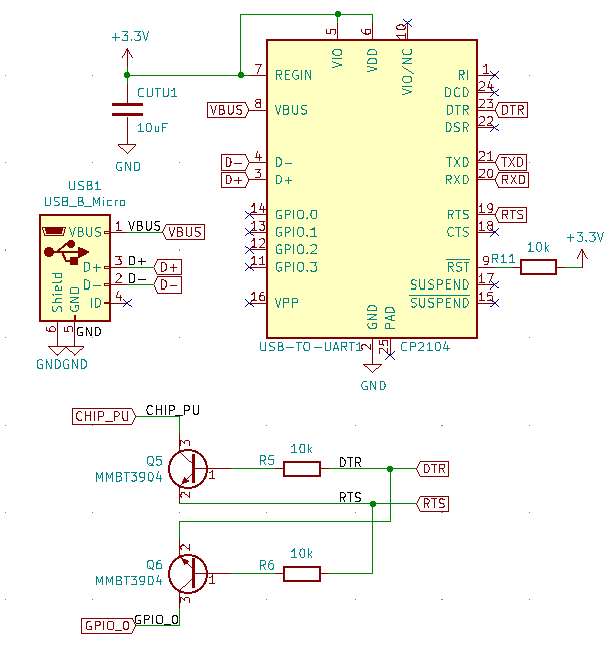
\includegraphics[width=0.75\textwidth]{graphics/shematics_usb.png}
	\caption{USB Anschluss}
	\label{pic: USB Anschluss}
\end{figure}
\begin{figure}[h!]
	\centering
	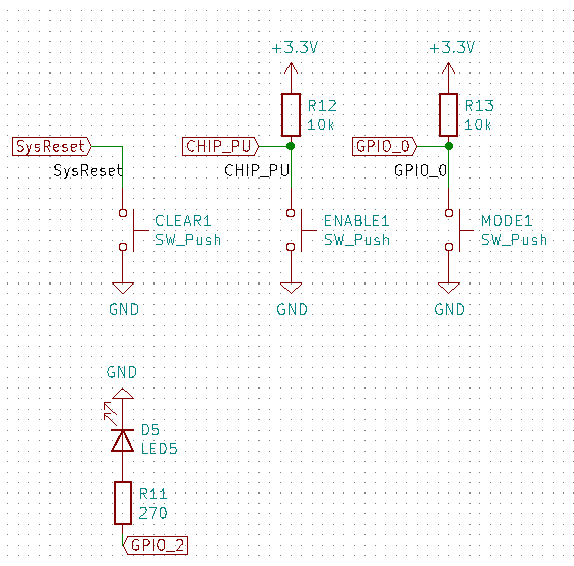
\includegraphics[width=0.6
	\textwidth]{graphics/shematics_sensor_buttons_LED.png}
	\caption{Buttons und LED auf Sensorbaustein}
	\label{pic: sensor_progrmmierbuttons}
\end{figure}
\subsubsection{Spannungsversorgung}
Der minimale Strom, welche die Spannungsquelle zur Verfügung stellen muss sind laut Datenblatt vom ESP32 500 mA, wobei im Normalbetrieb 80 mA und im WiFi Sendebtrieb 160 mA bis 260 mA gebraucht werden.
Um den Sensorbaustein mit 5 V zu versorgen, macht es aus Platz gründen Sinn den 230 V/AC zu 5 V/DC Wandler separat und nicht auf der Leiterplatte zu haben. Hier kommt beispielsweise der Mean Well RS-15-5 AC/DC infrage, welcher 90 V/AC bis 264 V/AC zu 5 V/DC bei max. 15 W bzw. 3 A wandeln kann. Dieser kostet bei Digi-Key momentan 9.47 Fr und ist noch dem unteren Preissegment zugeordnet, was aber immer noch relativ teuer ist im Vergleich zu den restlichen Komponenten. Da der Wandler separat zur Leiterplatte ist kann er jedoch immer noch im Nachhinein durch einen günstigeren mit vielleicht weniger Leistung ca. 5 W ausgetauscht werden.
Der Mikrocontroller benötigt 3.3 V, jedoch soll der Sensorbaustein mit 5V betrieben werden können. Hierfür wird einen Spannungswandler eingesetzt. Der ausgewählte AP1117S33CTR hat einen maximale Input Spannung von 15V, eine maximale Dropoutspannung von 1.2 V bei 800mA und ist, mit momentan 0.42\$ bei Digi-Key, günstig. Im Schema (Abb. \ref{pic: Wandler_Sensor}) erkennt man, dass sowohl über USB wie auch über einen Stecker den Print mit 5 V versorgt werden können. Eingebaut ist eine Sicherung die verhindern soll, dass bei einem Kurzschluss der Sensorbautein anfängt grossen Schaden zu nehmen oder schlimmeres.
\begin{figure}[h!]
	\centering
	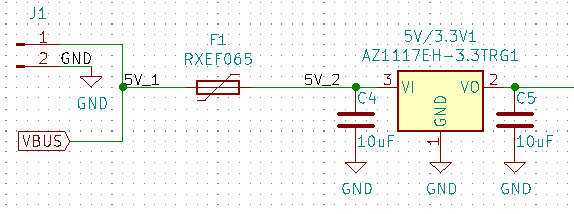
\includegraphics[width=0.7\textwidth]{graphics/shematics_sensor_33V.png}
	\caption{Spannungswandler Sensorbaustein}
	\label{pic: Wandler_Sensor}
\end{figure}
\subsubsection{Interface}
Der Sensorbaustein wird Taster und dazugehörige LEDs beinhalten, jedoch macht es Sinn diese auf einen separaten Print zur Verfügung zu stellen. Gründe hierfür sind der begrenzte Platz auf dem Hauptprint, separater Print kann als Frontplatte verwendet werden und bessere Integration der LEDs. Angedacht ist eine Frontplatte welche Touchsensoren, diese sind nichts anderes als dicke Leiterbahnen, beinhalten. Das einlesen der Touchsensoren gestaltet sich mit dem ESP32 äusserst einfach und läuft unabhängig vom WiFi, dies sei gesagt weil es z.B. Probleme gibt wenn der ADC2 und das WiFi gleichzeitig benutzt werden. Die LEDs könnten dann rückwärts montiert (reverse mounted LEDs) werden, welche durch die Leiterdplatte hindurchläuchten. In der Abbildung \ref{pic: Stecker_Sensor} sind die Steckverbindungen abgebildet, welche jeweils aus 4 Stecker für den Touch und LEDs bestehen, dazu kommen noch 3.3 V und GND Stecker sowie GPIO2, GPIO15, RXD und TXD Stecker, welche nützlich sind wenn man den Mikrocontroller über diese Schnittstelle programmieren oder einfach eine Verbindung haben möchte.
\begin{figure}[h!]
	\centering
	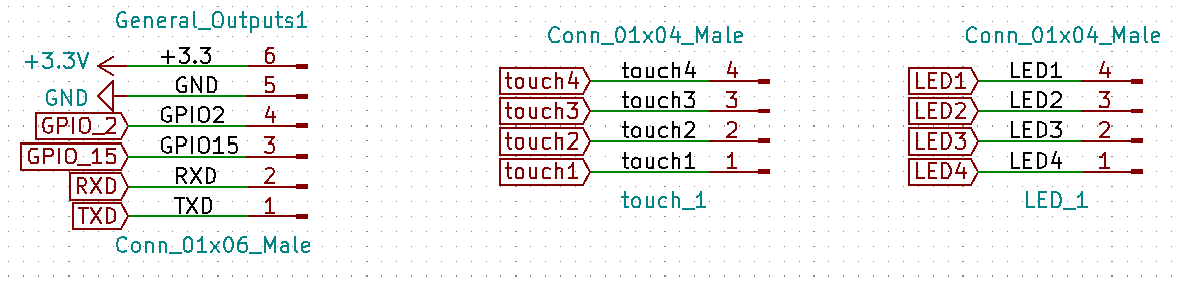
\includegraphics[width=0.8\textwidth]{graphics/shematics_sensor_stecker.png}
	\caption{Steckverbindungen Sensorbaustein}
	\label{pic: Stecker_Sensor}
\end{figure}
\subsubsection{Platzstudie}
Nun wird mittels einer Platzstudie überprüft ob der Sensorbaustein, mit den verwendeten Komponenten, wie eine Unterputzsteckdose eingebaut werden kann.
Im Bild \ref{pic: Montageplatte.png} ist eine Montageplatte für UP-Steckdosen abgebildet. Der blaue Kreis Zeigt dabei den Radius von 60 mm des Tasters bzw. Kleinkombination. Diese Masse wurden für die Dimensionen der Platine in Abbildung \ref{pic: pcb_sensor_dimensionen.png} übernommen. Abbildung \ref{pic: pcb_sensor_vorne} und \ref{pic: pcb_sensor_hinten} zeigen, wie die Komponenten auf der begrenzten Platine angeordnet werden können.

\begin{figure}[htb]
	\centering
	\begin{minipage}[t]{0.45\linewidth}
		\centering
		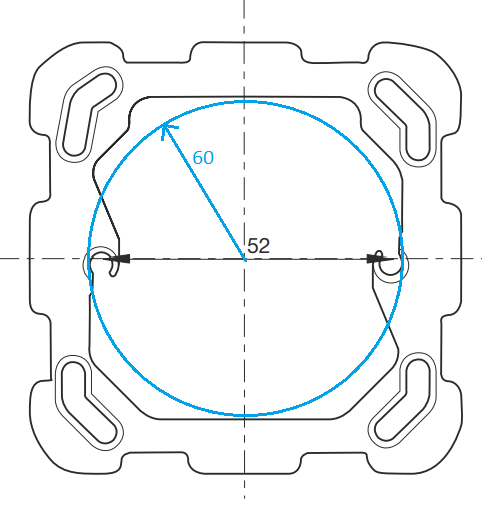
\includegraphics[width=0.9\textwidth]{graphics/Montageplatte.png}
		\caption{Montageplatte \cite{hager_hager_kat1_08_technik_d_2019} }
		\label{pic: Montageplatte.png}
	\end{minipage}% <- sonst wird hier ein Leerzeichen eingefügt
	\hfill
	\begin{minipage}[t]{0.45\linewidth}
		\centering
		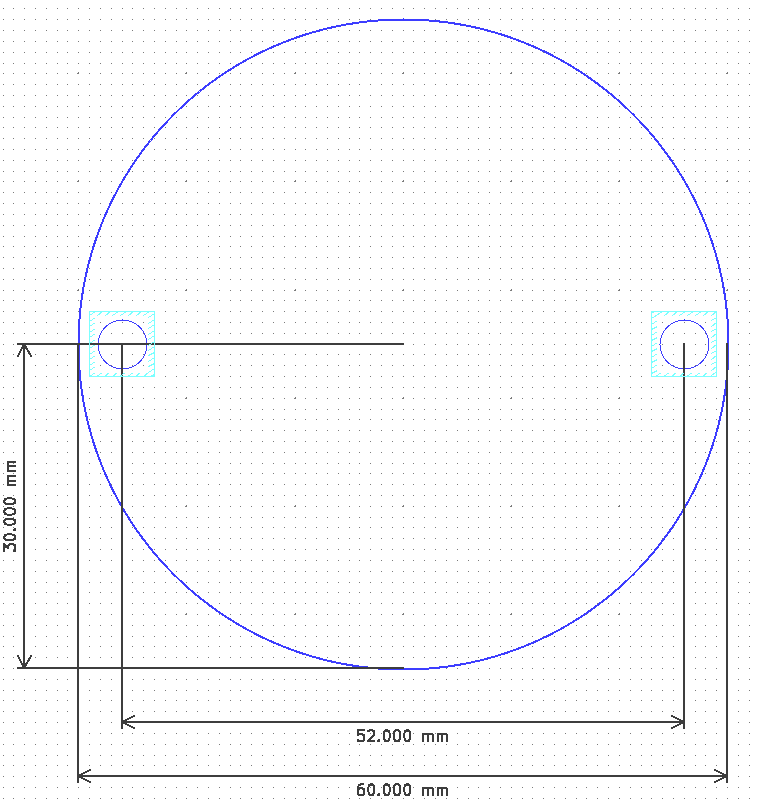
\includegraphics[width=0.90\textwidth]{graphics/pcb_sensor_dimensionen.png}
		\caption{PCB Sensorbaustein Dimensionen}
		\label{pic: pcb_sensor_dimensionen.png}
	\end{minipage}
\end{figure}

\begin{figure}[htb]
	\centering
	\begin{minipage}[t]{0.45\linewidth}
		\centering
	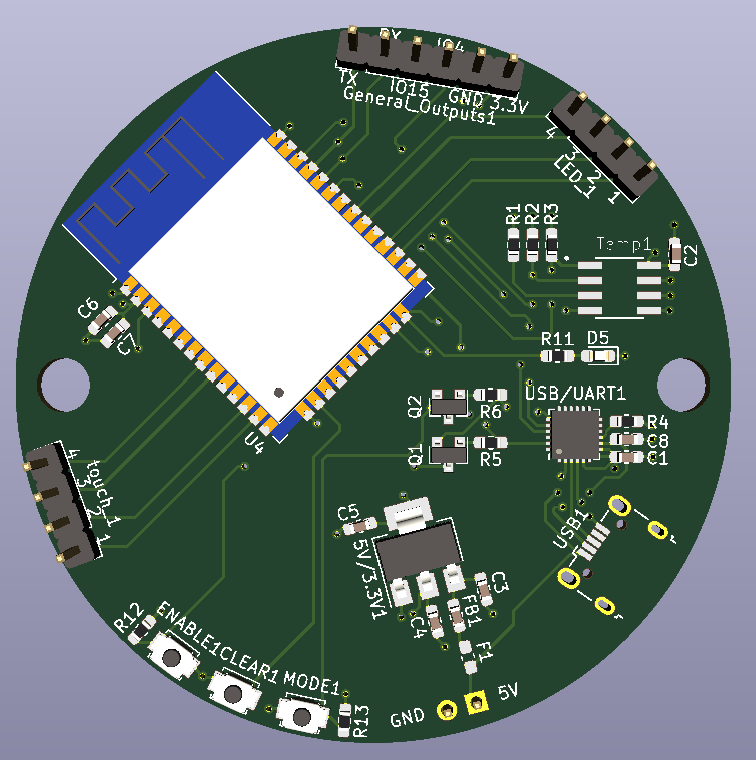
\includegraphics[width=0.90\textwidth]{graphics/pcb_sensor_vorne.png}
\caption{PCB Sensorbaustein von vorne}
\label{pic: pcb_sensor_vorne}
	\end{minipage}% <- sonst wird hier ein Leerzeichen eingefügt
	\hfill
	\begin{minipage}[t]{0.45\linewidth}
		\centering
	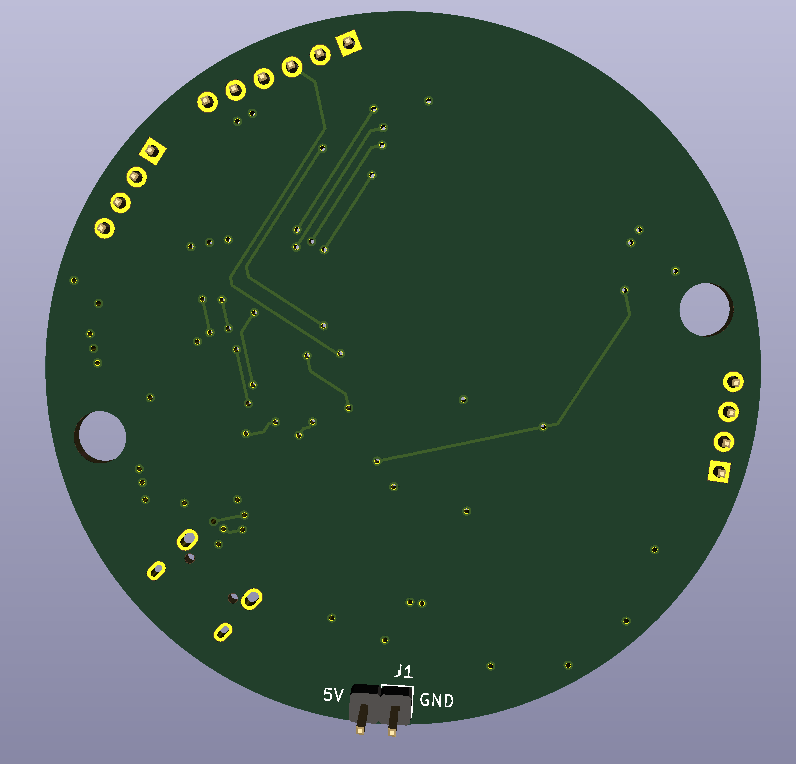
\includegraphics[width=0.90\textwidth]{graphics/pcb_sensor_hinten.png}
\caption{PCB Sensorbaustein von hinten}
\label{pic: pcb_sensor_hinten}
	\end{minipage}
\end{figure}





